\newpage
\section{Theoretical Analysis}
\label{sec:analysis}
In this section, the circuit shown in Figure~\ref{fig:Circuit} is analysed
theoretically. \\
At first, we are going to use the nodal method to compute voltages in all nodes and currents in all branches for t < 0.
After that, we will determine the equivalent resistance as seen from the capacitor terminals and the time constant, as well.
Then, using the equivalent resistance and the time constant discovered before, 
we are able to compute the natural solution of $v_6$(t) in the interval [0,20]ms and plot the result obtained.
We will also compute the forced solution of $v_6$(t) in the same interval, using phasors.
After, we are going to compute de final solution of $v_6$ and plot $v_6$(t) and $v_s$(t) in the interval of [-5,20]ms.
At last, we can plot $v_s$(f), $v_c$(f) and $v_6$(f) for frequency range 0,1Hz to 1MHz. 
To compute the values mentioned above, we use the following values (Resistances in Ohm, voltages in Volts, capacity in F, $K_b$ in S and $K_d$ in Ohms):
\begin{table}[h!]
\centering
\begin{small}
\caption{Given values by Python.} \label{Table1}
\begin{tabular}{|c|c|}
\hline
$R_1$ & \partialinput{1}{1}{tabelaVal.tex} \\
$R_2$ & \partialinput{2}{2}{tabelaVal.tex} \\
$R_3$  & \partialinput{3}{3}{tabelaVal.tex} \\
$R_4$ & \partialinput{4}{4}{tabelaVal.tex} \\
$R_5$  & \partialinput{5}{5}{tabelaVal.tex} \\
$R_6$ & \partialinput{6}{6}{tabelaVal.tex} \\
$R_7$ & \partialinput{7}{7}{tabelaVal.tex} \\
$V_s$ & \partialinput{8}{8}{tabelaVal.tex}\\
$C$ & \partialinput{9}{9}{tabelaVal.tex}\\
$K_b$ & \partialinput{10}{10}{tabelaVal.tex} \\
$K_d$ & \partialinput{11}{11}{tabelaVal.tex}\\
\hline
\end{tabular}
\end{small}
\end{table}

\newpage

\section{Nodal method for t < 0}
\label{t<0}

\noindent For t < 0, since u(t) = 0 and u(-t) = 1, vs = Vs. 
Also, we are considering that the voltage source has been turned on a long time ago for t < 0,therefore, all values are constant. 
The current flowing through the capacitor can be given by:
\begin{equation}
I_c = C\frac{dV_c}{dt}
  \label{eq:Ic}
\end{equation}

\noindent We can conclude that $v_c$ doesn't vary in time, so $I_c$ is 0 for t < 0.
There are seven unknown node voltages ($V_1$(t<0), $V_2$(t<0), $V_3$(t<0), $V_5$(t<0), $V_6$(t<0), $V_7$(t<0) and $V_8$(t<0)), 
so we need seven equations to compute these values.
\noindent In this analysis, we consider currents diverging from the node as positive values and currents converging as negative values and we used KCL, 
first on the nodes not connected to voltage sources and, after that, we have written additional equations for nodes related by voltage sources.

\noindent Starting with node 2, for this node, we considered all currents diverging, so we have this equation:
\begin{equation}
\frac{V_2(t<0) - V_1(t<0)}{R_1} + \frac{V_2(t<0) - V_5(t<0)}{R_3} + \frac{V_2(t<0) - V_3(t<0)}{R_2} = 0
  \label{eq:kvl_node2}
\end{equation}

\noindent In node 3, $I_b$ is converging and the current flowing through $R_2$ is diverging. $I_b$ equals to $K_b$$V_b$.
$V_B$ is equal to $V_2$ - $V_5$, due to the direction represented in the circuit for $R_3$ voltage:
\begin{equation}
\frac{V_3(t<0) - V_2(t<0)}{R_2} - K_b(V_2(t<0) - V_5(t<0)) = 0
  \label{eq:kvl_node3}
\end{equation}

\noindent Moving on to node 6, in which all currents are diverging and $I_c$ is 0, having this equation:
\begin{equation}
\frac{V_6(t<0) - V_5(t<0)}{R_5} + K_b(V_2(t<0) - V_5(t<0)) = 0
  \label{eq:kvl_node6}
\end{equation}

\noindent On the other side, in node 7, $I_d$ is converging and the current flowing through $R_7$ is diverging:
\begin{equation}
\frac{V_7(t<0) - V_8(t<0)}{R_7} + \frac{V_7(t<0)}{R_6} = 0
  \label{eq:kvl_node7}
\end{equation}

\noindent The next equation establish the relation between node 1 and GND voltages:
\begin{equation}
V_1 = V_s
  \label{eq:kvl_node1}
\end{equation}

\noindent The relation between nodes 5 and 8 is showed in the next equation:
\begin{equation}
V_5(t<0) - V_8(t<0) = \frac{-K_dV_7(t<0)}{R_6}
  \label{eq:kvl_node58}
\end{equation}

\noindent Since there is still an equation missing, we considered a super node containing $v_s$ branch and all currents diverging:
\begin{equation}
\frac{V_1(t<0) - V_2(t<0)}{R_1} - \frac{V_5(t<0)}{R_4} - \frac{V_7(t<0)}{R_6} = 0
  \label{eq:kvl_supernode}
\end{equation}

\noindent All these equations can be transformed in a matricial system as it is showed here:
$$ \left[ \begin{array}{ccccccc} -\frac{1}{R_1} & \frac{1}{R_1} + \frac{1}{R_2} + \frac{1}{R_3} & -\frac{1}{R_2} & -\frac{1}{R_3} & 0 & 0 & 0 \\
0 & -\frac{1}{R_2} - K_b & \frac{1}{R_2} & K_b & 0 & 0 & 0 \\
0 & K_b & 0 & -K_b -\frac{1}{R_5}& \frac{1}{R_5} & 0 & 0
\\ 0 & 0 & 0 & 0 & 0 & \frac{1}{R_6} + \frac{1}{R_7} & -\frac{1}{R_7}
\\ 1 & 0 & 0 & 0 & 0 & 0 & 0
\\ 0 & 0 & 0 & 1 & 0 & \frac{K_d}{R_6} & -1
\\ \frac{1}{R_1} & -\frac{1}{R_1} & 0 & -\frac{1}{R_4} & 0 & -\frac{1}{R_6} & 0\end{array} \right]
\left[ \begin{array}{c} V_1(t<0) \\ V_2(t<0) \\ V_3(t<0) \\ V_5(t<0) \\ V_6(t<0) \\ V_7(t<0) \\ V_8(t<0)\end{array} \right] = 
\left[ \begin{array}{c} 0 \\ 0 \\ 0 \\ 0 \\ V_s \\ 0 \\ 0\end{array} \right] $$

\noindent Solving the matricial system using Ocatve and the values given by Python, we have obtained the values showed above, in Table~\ref{Table4}.
\begin{table}[!h]
\centering
\begin{small}
\caption{Node voltages for t < 0.} \label{Table4}
\begin{tabular}{|c|c|}
\hline
Nodes Voltages & Values obtained (Volts)\\
\hline
$V_1$(t<0)           & \partialinput{1}{1}{tabela1.tex} \\
$V_2$(t<0)  & \partialinput{2}{2}{tabela1.tex}\\
$V_3$(t<0)   &      \partialinput{3}{3}{tabela1.tex} \\
$V_5$(t<0)  & \partialinput{4}{4}{tabela1.tex} \\
$V_6$(t<0)   & \partialinput{5}{5}{tabela1.tex} \\
$V_7$(t<0)    & \partialinput{6}{6}{tabela1.tex} \\
$V_8$(t<0)     &  \partialinput{7}{7}{tabela1.tex}\\
\hline
\end{tabular}
\end{small}
\end{table}

\noindent Having discovered nodes voltages, we need now to obtain the currents flowing in each resistance, 
$I_b$ and currents in $V_s$ and $V_d$ branches, with the following equations:

\begin{equation}
I_b = K_b(V_2(t<0) - V_5(t<0))
  \label{eq:Ib}
\end{equation}

\begin{equation}
R_1[i] = \frac{(V_1(t<0) - V_2(t<0))}{R_1}
  \label{eq: iR1}
\end{equation}

\begin{equation}
R_2[i] = \frac{(V_2(t<0) - V_3(t<0))}{R_2}
  \label{eq: iR2}
\end{equation}

\begin{equation}
R_3[i] = \frac{(V_2(t<0) - V_5(t<0))}{R_3}
  \label{eq: iR3}
\end{equation}

\begin{equation}
R_4[i] = \frac{-V_5(t<0)}{R_4}
  \label{eq: iR4}
\end{equation}

\begin{equation}
R_5[i] = \frac{(V_5(t<0) - V_6(t<0))}{R_5}
  \label{eq: iR5}
\end{equation}

\begin{equation}
R_6[i] = \frac{-V_7(t<0)}{R_6}
  \label{eq: iR6}
\end{equation}

\begin{equation}
R_7[i] = \frac{V_7(t<0) - V_8(t<0)}{R_7}
  \label{eq: iR7}
\end{equation}

\begin{equation}
v_s[i] = -R_1[i]
  \label{eq: ivs}
\end{equation}

\begin{equation}
V_d[i] = R_3[i] + R_4[i] - R_5[i]
  \label{eq: ivd}
\end{equation}

\begin{table}[h!]
\centering
\begin{small}
\caption{Branch currents for t < 0.} \label{Table5}
\begin{tabular}{|c|c|}
\hline
Branch currents & Values obtained (Ampers)\\
\hline
$I_b$ & \partialinput{8}{8}{tabela1.tex} \\
$R_1[i]$  & \partialinput{9}{9}{tabela1.tex}\\
$R_2[i]$   & \partialinput{10}{10}{tabela1.tex} \\
$R_3[i]$ & \partialinput{11}{11}{tabela1.tex} \\
$R_4[i]$  & \partialinput{12}{12}{tabela1.tex} \\
$R_5[i]$ & \partialinput{13}{13}{tabela1.tex}\\
$R_6[i]$   & \partialinput{14}{14}{tabela1.tex} \\
$R_7[i]$ & \partialinput{15}{15}{tabela1.tex} \\
$v_s[i]$   & \partialinput{16}{16}{tabela1.tex} \\
$V_d[i]$ & \partialinput{17}{17}{tabela1.tex} \\
\hline
\end{tabular}
\end{small}
\end{table}

\newpage
\section{Equivalent resistance and time constant}
\label{t=0}

\noindent In this section, we analyse the circuit for t = 0 and, consequently, $v_s$ equals 0, as well as $V_1$. 
To compute the equivalent resistance as seen from the capacitor terminals and the time constant, we replace the capacitor with a voltage source:
\begin{equation}
V_x = V_6(t<0) - V_8(t<0),
  \label{eq: Vx}
\end{equation}
where $V_6$(t<0) and $V_8$(t<0) are the values computed in Section~\ref{t<0}. 
\noindent In a circuit with dependent sources, as the one in analysis, we can't turn off all sources to compute the equivalent resistance as seen from one component.
Having this said, We need to discover the equivalent current, flowing through the capacitor, which we named $I_x$, 
in this case, and the equivalent voltage, $V_x$, which we know already from equation~\ref{eq: Vx}).
Using this procesure, we also ensure the continuity of the capacitor voltage. \\
\noindent Hence, we now have six voltages to compute ($V_2$(t=0), $V_3$(t=0), $V_5$(t=0), $V_6$(t=0), $V_7$(t=0) and $V_8$(t=0)), needing, thus, six equations, 
some similar to the ones from Section ~\ref{t<0}.
In node 2, 3 and 7 and in the supernode equation, the only change is that now $V_1$(t=0) is 0:
\begin{equation}
\frac{V_2(t=0)}{R_1} + \frac{V_2(t=0) - V_5(t=0)}{R_3} + \frac{V_2(t=0) - V_3(t=0)}{R_2} = 0
  \label{eq:2kvl_node2}
\end{equation}

\begin{equation}
\frac{V_3(t=0) - V_2(t=0)}{R_2} - K_b(V_2(t=0) - V_5(t=0)) = 0
  \label{eq:2kvl_node3}
\end{equation}

\begin{equation}
\frac{V_7(t=0) - V_8(t=0)}{R_7} + \frac{V_7(t=0)}{R_6} = 0
  \label{eq:3kvl_node7}
\end{equation}

\begin{equation}
-\frac{V_2(t=0)}{R_1} - \frac{V_5(t=0)}{R_4} - \frac{V_7(t=0)}{R_6} = 0
  \label{eq:supernode2}
\end{equation}

\noindent Moving to the new equation, that relates voltages of nodes 6 and 8, which are now connected by a voltage source $V_x$:
\begin{equation}
V_6(t=0) - V_8(t=0) = V_x
  \label{eq:V68}
\end{equation}

\noindent These equations can be transformed in the following matricial system:
$$ \left[ \begin{array}{cccccc} \frac{1}{R_1} + \frac{1}{R_2} + \frac{1}{R_3} & -\frac{1}{R_2} & -\frac{1}{R_3} & 0 & 0 & 0 \\
-\frac{1}{R_2} - K_b & \frac{1}{R_2} & K_b & 0 & 0 & 0 
\\ 0 & 0 & 0 & 0 & \frac{1}{R_6} + \frac{1}{R_7} & -\frac{1}{R_7}
\\ 0 & 0 & 1 & 0 & \frac{K_d}{R_6} & -1
\\ -\frac{1}{R_1} & 0 & -\frac{1}{R_4} & 0 & -\frac{1}{R_6} & 0
\\ 0 & 0 & 0 & 1 & 0 & -1\end{array} \right]
\left[ \begin{array}{c} V_2(t=0) \\ V_3(t=0) \\ V_5(t=0) \\ V_6(t=0) \\ V_7(t=0) \\ V_8(t=0)\end{array} \right] = 
\left[ \begin{array}{c} 0 \\ 0 \\ 0 \\ 0 \\ 0 \\ V_x\end{array} \right] $$

\noindent Having solved this system in Octave, we have obtained the following voltages for each node:
\begin{table}[!h]
\centering
\begin{small}
\caption{Node voltages for t = 0.} \label{Table5}
\begin{tabular}{|c|c|}
\hline
Nodes Voltages & Values obtained (Volts)\\
\hline
$V_2$(t=0)  & \partialinput{1}{1}{tabela2.tex}\\
$V_3$(t=0)   & \partialinput{2}{2}{tabela2.tex} \\
$V_5$(t=0)   & \partialinput{3}{3}{tabela2.tex} \\
$V_6$(t=0)    & \partialinput{4}{4}{tabela2.tex} \\
$V_7$(t=0)     & \partialinput{5}{5}{tabela2.tex} \\
$V_8$(t=0)     &  \partialinput{6}{6}{tabela2.tex}\\
\hline
\end{tabular}
\end{small}
\end{table}

\noindent Having discovered nodes voltages, we need now to obtain the currents flowing in each resistance, 
$I_b$ and currents in $V_s$ and $V_d$ branches, with the following equations:

\begin{equation}
I_b = K_b(V_2(t=0) - V_5(t=0))
  \label{eq:Ib}
\end{equation}

\begin{equation}
R_1[i] = -\frac{V_2(t=0)}{R_1}
  \label{eq: iR10}
\end{equation}

\begin{equation}
R_2[i] = \frac{(V_2(t=0) - V_3(t=0))}{R_2}
  \label{eq: iR20}
\end{equation}

\begin{equation}
R_3[i] = \frac{(V_2(t=0) - V_5(t=0))}{R_3}
  \label{eq: iR30}
\end{equation}

\begin{equation}
R_4[i] = \frac{-V_5(t=0)}{R_4}
  \label{eq: iR40}
\end{equation}

\begin{equation}
R_5[i] = \frac{(V_5(t=0) - V_6(t=0))}{R_5}
  \label{eq: iR50}
\end{equation}

\begin{equation}
R_6[i] = \frac{-V_7(t=0)}{R_6}
  \label{eq: iR60}
\end{equation}

\begin{equation}
R_7[i] = \frac{V_7(t=0) - V_8(t=0)}{R_7}
  \label{eq: iR70}
\end{equation}

\begin{equation}
v_s[i] = -R_1[i]
  \label{eq: ivs0}
\end{equation}

\begin{equation}
V_d[i] = R_3[i] + R_4[i] - R_5[i]
  \label{eq: ivd0}
\end{equation}

\begin{table}[h!]
\centering
\begin{small}
\caption{Branch currents for t = 0.} \label{Table100}
\begin{tabular}{|c|c|}
\hline
Branch currents & Values obtained (Ampers)\\
\hline
$I_b$ & \partialinput{11}{11}{tabela2.tex} \\
$R_1[i]$  & \partialinput{12}{12}{tabela2.tex}\\
$R_2[i]$   & \partialinput{13}{13}{tabela2.tex} \\
$R_3[i]$ & \partialinput{14}{14}{tabela2.tex} \\
$R_4[i]$  & \partialinput{15}{15}{tabela2.tex} \\
$R_5[i]$ & \partialinput{16}{16}{tabela2.tex}\\
$R_6[i]$   & \partialinput{17}{17}{tabela2.tex} \\
$R_7[i]$ & \partialinput{18}{18}{tabela2.tex} \\
$v_s[i]$   & \partialinput{19}{19}{tabela2.tex} \\
$V_d[i]$ & \partialinput{20}{20}{tabela2.tex} \\
\hline
\end{tabular}
\end{small}
\end{table}

\noindent After this, we are able to compute $I_x$, since this current is given by, using KCL in node 6:
\begin{equation}
I_x = -\frac{(V_6(t=0) - V_5(t=0))}{R_5} - K_b(V_2(t=0) - V_5(t=0))
  \label{eq:Ix}
\end{equation}

\noindent At last, we calculated $R_{eq}$, in Ohms, and $\tau$, in seconds, using the following equations:
\begin{equation}
R_{eq} = |\frac{V_x}{I_x}|
  \label{eq:Req}
\end{equation}

\begin{equation}
\tau = R_{eq}C
  \label{eq:tau}
\end{equation}

\noindent The results obtained are showed in Table~\ref{Table6}:
\begin{table}[!h]
\centering
\begin{small}
\caption{Equivalent resistance and time constant} \label{Table6}
\begin{tabular}{|c|c|}
\hline
$V_X$  & \partialinput{7}{7}{tabela2.tex}\\
$I_x$   & \partialinput{8}{8}{tabela2.tex} \\
$R_{eq}$   & \partialinput{9}{9}{tabela2.tex} \\
$\tau$    & \partialinput{10}{10}{tabela2.tex} \\
\hline
\end{tabular}
\end{small}
\end{table}

\newpage
\section{Natural solution $v_6n$(t)}
In this section, the main goal is to compute the natural solution of $v_{6n}$(t). For that, we used the general solution given by:
\begin{equation}
v_{6n}(t) = V_6(+\infty) + (V_6(t=0) - V_6(+\infty))e^{\frac{-t}{\tau}}
  \label{eq:v6ncomplete}
\end{equation}
In this circuit, we can conclude that the capacitor begins charged and, as time goes by, it discharges. Also, in t = 0, $V_8$ equals 0. 
For both reasons, $v_6(+\infty)$ equals 0, meaning that $v_{6n}$(t) can be computed with the following equation:
\begin{equation}
v_{6n}(t) = V_6(t=0)e^{\frac{-t}{\tau}}
  \label{eq:v6nfinal}
\end{equation}
It can also be written, using $V_x$ and $V_8$(t=0):
\begin{equation}
v_{6n}(t) = (V_x + V_8(t=0))e^{\frac{-t}{\tau}}
  \label{eq:v6nwithv8vx}
\end{equation}
Since $V_8$ equals 0, as mentioned before, we can simply write:
\begin{equation}
v_{6n}(t) = V_xe^{\frac{-t}{\tau}}
  \label{eq:v6nwithvx}
\end{equation}
To finish this section, we plot this function in the interval of [0,20]ms.
\begin{figure}[h!] \centering
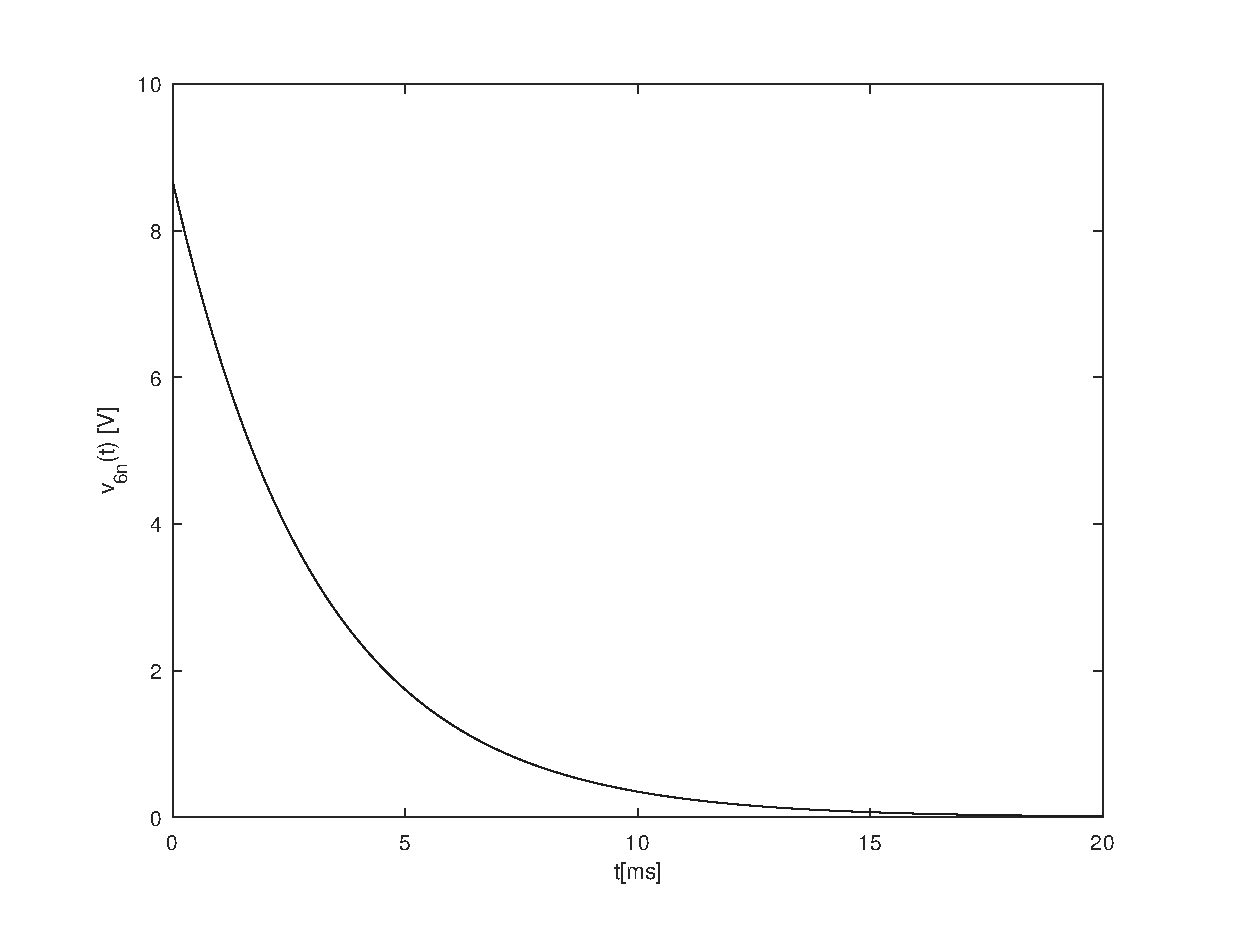
\includegraphics[width=0.8\linewidth]{v6n.eps}
\caption{Natural Solution $v_{6n}(t)$ in [0,20]ms.}
\label{fig:v6n}
\end{figure}

\newpage
\section{Forced solution $v_6f$(t)}
In this section, the main goal is to compute the forced solution of $v_{6f}$(t). First, we have to compute the complex amplitudes of voltages in each node, using the node method, in the same way we did previously in Section~\ref{t<0}, but considering, this time, the capacitor and the currents flowing through it, using its impedance. 
Hence, the only equation that is different from those written in Section~\ref{t<0} is the one referring to node 6. In the capacitor, we have:
\begin{equation}
Z_c = \frac{1}{iwc}
\label{eq:impedance}
\end{equation}

\begin{equation}
v_c = I_cZ_c
\label{eq:capacitor}
\end{equation}

\noindent Therefore, in node 6, considering all currents diverging and $v_c$ = $V_6$(t > 0) - $V_8$(t > 0), KCL can be given by the following equation:
\begin{equation}
\frac{V_6(t>0) - V_5(t>0)}{R_5} + K_b(V_2(t>0) - V_5(t>0)) + \frac{V_6(t>0) - V_8(t>0)}{Z_c}= 0
  \label{eq:node6}
\end{equation}
This method gives us enough equations to build a matricial system to solve, with seven voltages to compute and seven equations:
$$ \left[ \begin{array}{ccccccc} -\frac{1}{R_1} & \frac{1}{R_1} + \frac{1}{R_2} + \frac{1}{R_3} & -\frac{1}{R_2} & -\frac{1}{R_3} & 0 & 0 & 0 \\
0 & -\frac{1}{R_2} - K_b & \frac{1}{R_2} & K_b & 0 & 0 & 0 \\
0 & K_b & 0 & -K_b -\frac{1}{R_5}& \frac{1}{R_5} + \frac{1}{Z_c} & 0 & 0
\\ 0 & 0 & 0 & 0 & 0 & \frac{1}{R_6} + \frac{1}{R_7} & -\frac{1}{R_7}
\\ 1 & 0 & 0 & 0 & 0 & 0 & 0
\\ 0 & 0 & 0 & 1 & 0 & \frac{K_d}{R_6} & -1
\\ \frac{1}{R_1} & -\frac{1}{R_1} & 0 & -\frac{1}{R_4} & 0 & -\frac{1}{R_6} & 0\end{array} \right]
\left[ \begin{array}{c} V_1(t>0) \\ V_2(t>0) \\ V_3(t>0) \\ V_5(t>0) \\ V_6(t>0) \\ V_7(t>0) \\ V_8(t>0)\end{array} \right] = 
\left[ \begin{array}{c} 0 \\ 0 \\ 0 \\ 0 \\ V_s \\ 0 \\ 0\end{array} \right] $$

\noindent Solving the given system, we obtain the complex amplitude voltages in all nodes, including node 6. The results are expressed in the following table:
\begin{table}[h!]
\centering
\begin{small}
\caption{Complex Amplitude Voltages In All Nodes (Volts).} \label{Table9}
\begin{tabular}{|c|c|}
\hline
$V_1$(t > 0) & \partialinput{1}{1}{tabela6.tex}$e^{\partialinput{8}{8}{tabela6.tex} i}$\\
$V_2$(t > 0) & \partialinput{2}{2}{tabela6.tex}$e^{\partialinput{9}{9}{tabela6.tex} i}$\\
$V_3$(t > 0) & \partialinput{3}{3}{tabela6.tex}$e^{\partialinput{10}{10}{tabela6.tex} i}$\\
$V_5$(t > 0) & \partialinput{4}{4}{tabela6.tex}$e^{\partialinput{11}{11}{tabela6.tex} i}$\\
$V_6$(t > 0) & \partialinput{5}{5}{tabela6.tex}$e^{\partialinput{12}{12}{tabela6.tex} i}$\\
$V_7$(t > 0) & \partialinput{6}{6}{tabela6.tex}$e^{\partialinput{13}{13}{tabela6.tex} i}$\\
$V_8$(t > 0)& \partialinput{7}{7}{tabela6.tex}$e^{\partialinput{14}{14}{tabela6.tex} i}$\\
\hline
\end{tabular}
\end{small}
\end{table}

\noindent To obtain the forced solution of $v_6$, the following expression can be used:
\begin{equation}
V_{6f}(t) = V_6(t > 0) sin(wt)
  \label{eq:v6fcomplete}
\end{equation}


\newpage
\section{Total solution $v_6$(t)}
To obtain the total solution for the voltage of node 6 and of the voltage source $v_s$, in the given time range, 
[-5,20ms] we need to consider three cases for t<0, t=0 and t>0.
In the first case, $v_s$ equals $V_s$ and $v_6$ is the voltage we obtained in Section~\ref{t<0}.
In the moment t = 0, $v_s$ also equals $V_s$, since sin(0) = 0, and $v_6$ is the value obtained in Section~\ref{t=0}.
The third and last case, $v_s$ equals $sin(2\pi*f*t)$, as we can see by the expression in Figure~\ref{fig:Circuit}, but to compute $V_6$ we have to consider the natural and forced solution:
\begin{equation}
{V_6}(t) = V_{6f}(t) + V_{6n}(t)
\label{eq:v6fcomplete}
\end{equation}
\noindent Finally, these three separate conditions can be summed up in the following graph, where $v_s$ and $v_6$ are plotted:
\begin{figure}[h!] \centering
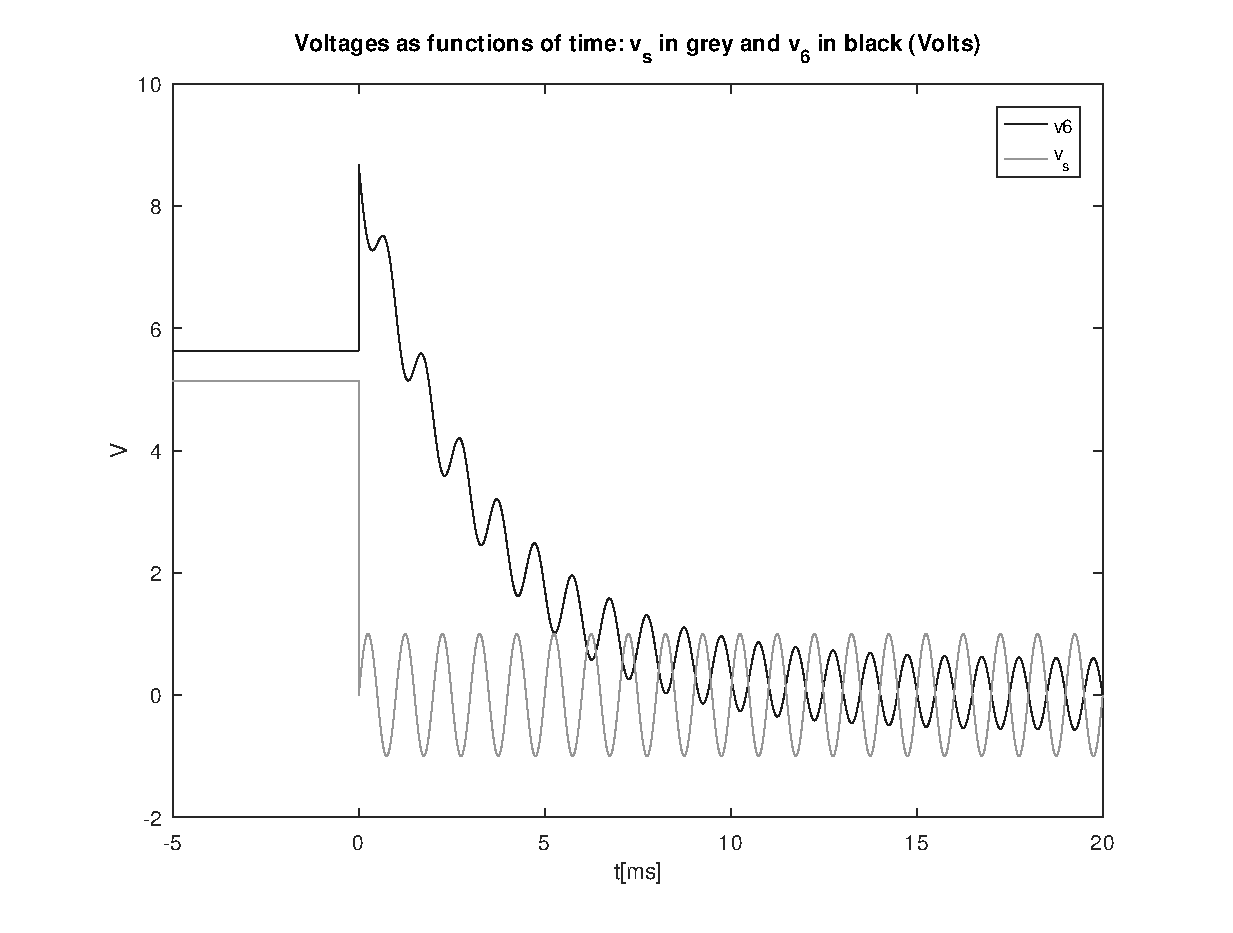
\includegraphics[width=0.8\linewidth]{v6.eps}
\caption{$v_{s}(t)$ and Total Solution $v_{6}(t)$ in [-5,20]ms for f = 1kHz.}
\label{fig:v6t}
\end{figure}

\newpage
\section{Frequency Responses - $v_s$(f), $v_c$(f), $v_6$(f)}
In this section we need to determine how the complex voltages $v_c$, $v_s$ and $v_6$ vary with different frequencies 
and plot them in the same graph. As $v_1$ equals $v_s$ we do not have to include it in our next matricial system. 
Also, if we look at the equations on it, the only voltages that depend on the frequency are $v_6$ and $v_8$. 
If we rearrange that system to take that into account, we only need 4 equations to obtain the values that do not depend on the frequency. 
That way, the following matrix can be found, using nodal method:

$$ \left[ \begin{array}{cccc} - K_b -\frac{1}{R_2}  & \frac{1}{R_2} & K_b & 0 \\
\frac{1}{R_3} - K_b & 0 & K_b -\frac{1}{R_3}-\frac{1}{R_4} & -\frac{1}{R_6} \\
K_b-\frac{1}{R_1}-\frac{1}{R_3} & 0 & \frac{1}{R_3}-K_b & 0 
\\ 0 & 0 & 1 & \frac{K_d - R_7}{R_6}-1\end{array} \right]
\left[ \begin{array}{c} V_2 \\ V_3 \\ V_5 \\ V_7 \end{array} \right] = 
\left[ \begin{array}{c} 0 \\ 0 \\ -v_sphasor \\ 0 \end{array} \right] $$
For the matrix above, we have to take into account that:
\begin{equation}
v_sphasor = e^{-i\pi/2}
\label{eq:vsphasor}
\end{equation}

Now that we have computed all the node voltages that are not dependent on the frequency, 
we are able to compute $v_6$ and $v_8$ and then $v_c$, using the following equations:
\begin{equation}
v_8 = R_7V_7(\frac{1}{R_1} + \frac{1}{R_6});
\label{eq:V_8}
\end{equation}

\begin{equation}
v_6 = \frac{V_5(K_b + \frac{1}{R_5}) - K_bV_2 + \frac{v_8}{Z_c}}{\frac{1}{R_5} + \frac{1}{Z_c}} 
\label{eq:V_6}
\end{equation}

\begin{equation}
v_c = v_6 - v_8
\label{eq:V_c}
\end{equation}

At last, we choose [-90,90] degrees to be the interval for the phases computed. 
Plots of magnitude (dB) and phase (degrees) of $v_c$, $v_6$ and $v_s$, in function of frequency, are showed next.
\begin{figure}[h!] \centering
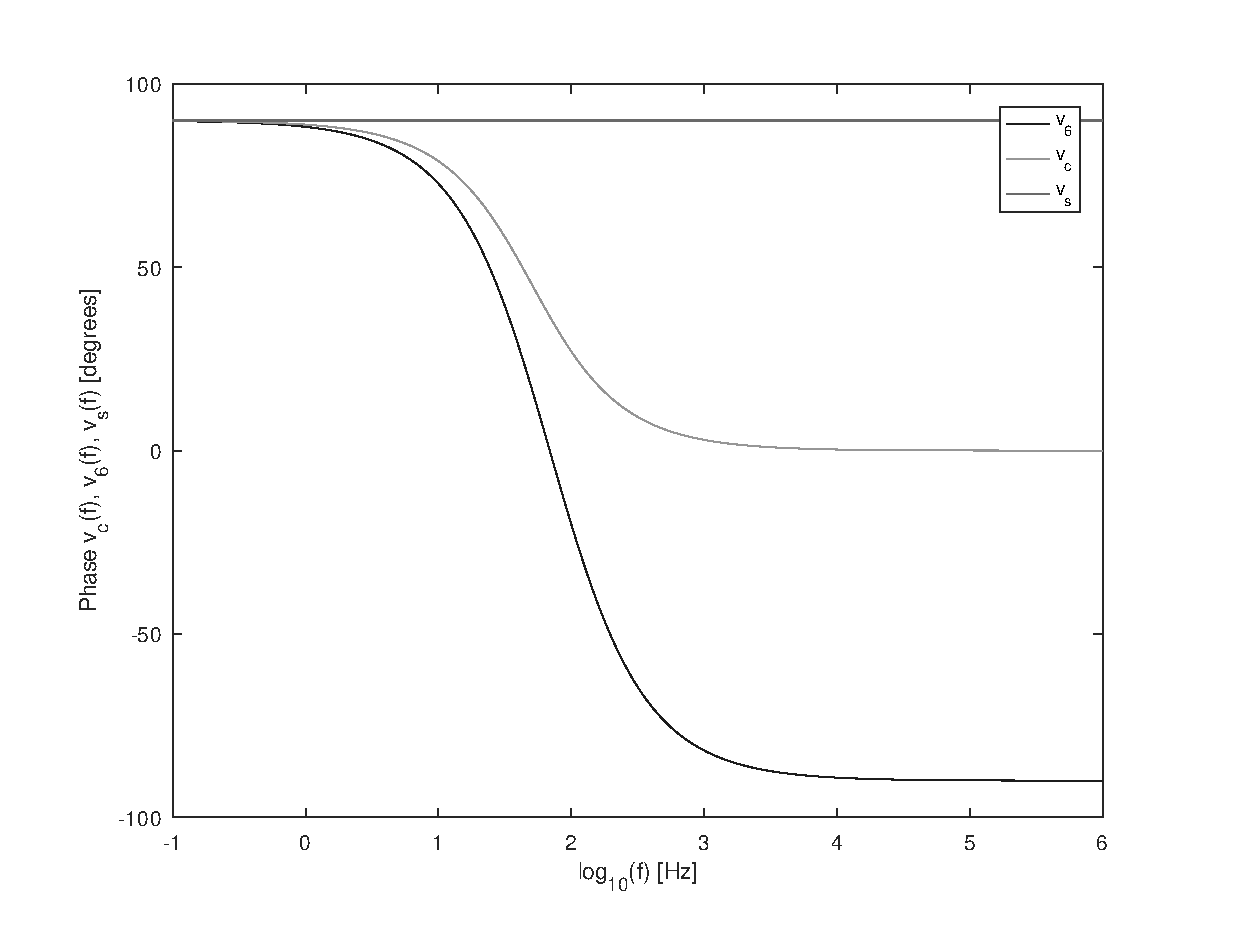
\includegraphics[width=0.7\linewidth]{Phase(degrees).eps}
\caption{Phase of $v_s$, $v_c$ and $v_6$ in function of frequency (Degrees).}
\label{fig:phase}
\end{figure}

\begin{figure}[h!] \centering
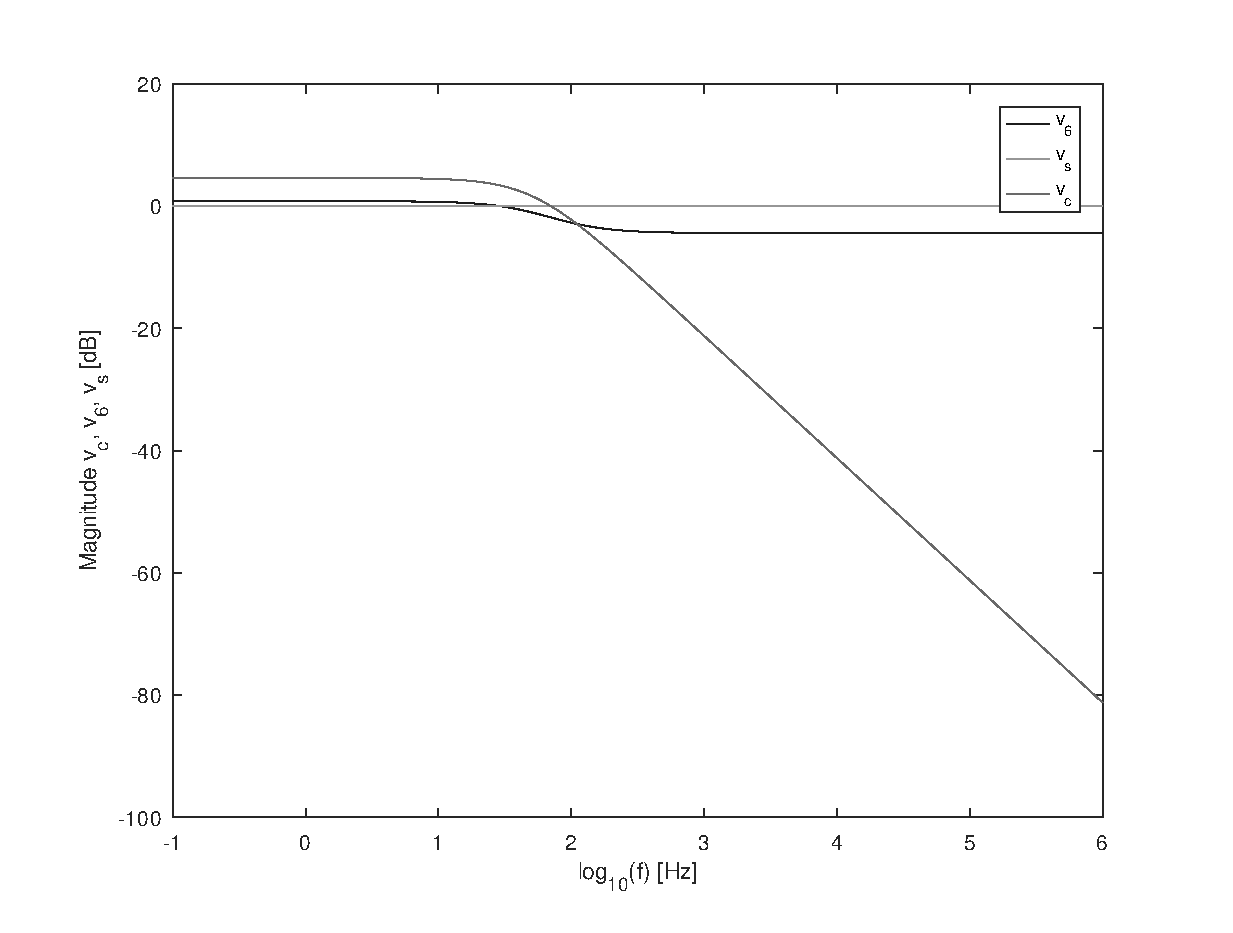
\includegraphics[width=0.7\linewidth]{MagnitudedB.eps}
\caption{Magnitude of $v_s$, $v_c$ and $v_6$ in function of frequency (dB).}
\label{fig:magnitude}
\end{figure}

